\section{Introduction to Artificial Neural Network}



\subsection{Autodiff}

\cindex{Autodiff} is neither a numerical nor symbolic differentiation. It use numerical method calculation and use symbolic rules for differentiation, so it is partly symbolic and partly numerical. See \cite{GunesBaydin2018} for more details.


One example is $f(x_1, x_2) = \log{x_1} + x_1 x_2 - \sin{x_2}$. The computation graph is:

\begin{figure}[H]
\centering	
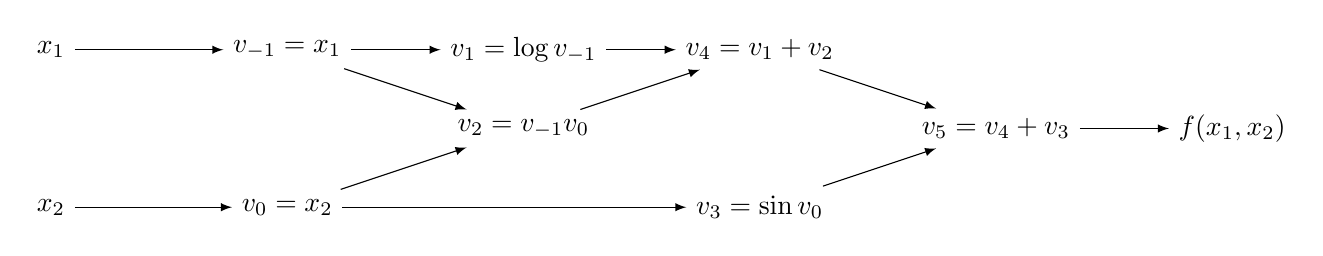
\begin{tikzpicture}
    \node (x2) at (0,0) {$x_2$};
    \node (x1) at (0,2) {$x_1$};
    \node (v0) at (3,0) {$v_0 = x_2$};
    \node (v_1) at (3,2) {$v_{-1} = x_1$};
    \node (v2) at (6,1) {$v_2 = v_{-1} v_0$};
    \node (v1) at (6,2) {$v_1 = \log{v_{-1}}$};
    \node (v3) at (9,0) {$v_3 = \sin{v_0}$};
    \node (v4) at (9,2) {$v_4 = v_1 + v_2$};
    \node (v5) at (12,1) {$v_5 = v_4 + v_3$};
    \node (final) at (15,1) {$f(x_1,x_2)$};
    \draw [-latex] (x2) -- (v0);
    \draw [-latex] (v0) -- (v3);
    \draw [-latex] (v3) -- (v5);  
    \draw [-latex] (x1) -- (v_1);
    \draw [-latex] (v_1) -- (v1);  
    \draw [-latex] (v1) -- (v4);
    \draw [-latex] (v4) -- (v5);  
    \draw [-latex] (v_1) -- (v2);
    \draw [-latex] (v2) -- (v4);
    \draw [-latex] (v0) -- (v2);
    \draw [-latex] (v5) -- (final);
\end{tikzpicture}
\caption{$f(x_1, x_2) = \log{x_1} + x_1 x_2 - \sin{x_2}$}
\end{figure}


In general there are two autodiff methods: forward mode and backpropagation. In forward mode, the derivative is the intermediary nodes against all input nodes while in backpropagation the derivative is the final node against all intermediary nodes.



\subsubsection{Forward Mode}

There are $1+n$ passes in forward mode:
\begin{enumerate}
    \item a forward evaluation of all node values. Table \ref{forwardprimaltracetable} shows the forward example.
    \item $n$ forward derivative calculation for all $n$ input features. For the $i$-th input feature, the derivatives of all $\dot{v}$ is calculated in Table \ref{forwardtangenttrace}.
\end{enumerate}

\begin{table}[H]
\centering
    \begin{tabular}{lll}
        $v_{-1}$ & $= x_1$ & $ = 2$ \\
        $v_0$ & $= x_2$ & $=5$ \\
        $v_1$ & $=\log{v_{-1}}$ & $= \log{2}$ \\
        $v_2$ & $=v_{-1} \times v_0$ & $= 2 \times 5 $\\
        $v_3$ & $=\sin{v_0}$ & $=\sin{5}$\\
        $v_4$ & $=v_1 + v_2$ & $=0.693+10$ \\
        $v_5$ & $=v_4 - v_3$ & $=10.693 + 0.959$ \\
        $y$ & $=v_5$ & $=11.652$ \\
    \end{tabular}
\caption{Forward Primal Trace}
\label{forwardprimaltracetable}
\end{table}


\begin{table}[H]
\centering
    \begin{tabular}{lll}
        $\dot{v}_{-1}$ & $= \dot{x}_1$ & $ = 1$ \\
        $\dot{v}_0$ & $= \dot{x}_2$ & $=0$ \\
        $\dot{v}_1$ & $= \displaystyle \frac{\dot{v}_{-1}}{v_{-1}}$ & $=\displaystyle \frac{1}{2}$ \\
        $\dot{v}_2$ & $=\dot{v}_{-1} \times v_0 + v_{-1} \times \dot{v}_0$ & $= 1 \times 5 + 0 \times 2$\\
        $\dot{v}_3$ & $=\dot{v}_0 \times \cos{v_0}$ & $=0 \times \cos{5}$ \\
        $\dot{v}_4$ & $=\dot{v}_1 + \dot{v}_2$ & $= 0.5 + 5$ \\
        $\dot{v}_5$ & $=\dot{v}_4 - \dot{v}_3$ & $= 5.5 - 0$ \\
        $\dot{y}$ & $=\dot{v}_5$ & $= 5.5$ \\
    \end{tabular}
\caption{Forward Tangent (Derivative) Trace}
\label{forwardtangenttrace}
\end{table}

Forward mode is expensive because it needs to run a pass for each input feature.


\subsubsection{Backpropogation}

\cindex{Backpropagation} only needs 2 passes over the calculation graph:
\begin{enumerate}
    \item a forward evaluation of all node values. The same as forward mode. Table \ref{forwardprimaltracetable} shows the forward example.
    \item a backward derivative calculation of all nodes in calculation graph. Table \ref{reverseadjointtrace} shows the backward example.
\end{enumerate}

In the backward derivative calculation, all derivatives are calculated against final result $y$. According to calculas, we have:
\begin{equation}
    \dpd{y}{v_0} = \dpd{y}{v_2} \dpd{v_2}{v_0} + \dpd{y}{v_3} \dpd{v_3}{v_0}
\end{equation}

Let $\bar{v} = \pd{y}{v}$. We have:
\begin{equation}
    \bar{v}_0 = \bar{v}_2 \dpd{v_2}{v_0} + \bar{v}_3 \dpd{v_3}{v_0}
\end{equation}

So the final result could calculated by backward propagation. Table \ref{reverseadjointtrace} gives an example.

\begin{table}[H]
\centering
    \begin{tabular}{llll}
        $\bar{v}_5$ & $=\bar{y}$ && $= 1$ \\
        $\bar{v}_4$ & $=\bar{v}_5 \pd{v_5}{v_4}$ & $=\bar{v}_5 \times 1$ & $=1$ \\
        $\bar{v}_3$ & $=\bar{v}_5 \pd{v_5}{v_3}$ & $=\bar{v}_5 \times (-1)$ & $=-1$ \\
        $\bar{v}_2$ & $=\bar{v}_4 \pd{v_4}{v_2}$ & $=\bar{v}_4 \times 1$ & $=1$ \\
        $\bar{v}_1$ & $=\bar{v}_4 \pd{v_4}{v_1}$ & $=\bar{v}_4 \times 1$ & $=1$ \\
        $\bar{v}_0$ & $=\bar{v}_3 \pd{v_3}{v_0}$ & $=\bar{v}_3 \times \cos{v_0}$ & $=-0.284$ \\
        $\bar{v}_{-1}$ & $=\bar{v}_2 \pd{v_2}{v_{-1}}$ & $=\bar{v}_2 \times v_0$ & $=5$ \\
        $\bar{v}_0$ & $=v_0 + \bar{v}_2 \pd{v_2}{v_0}$ & $=\bar{v}_0 +\bar{v}_2 \times v_{-1}$ & $=1.716$ \\
        $\bar{v}_{-1}$ & $=v_{-1} + \bar{v}_1 \pd{v_1}{v_{-1}}$ & $=\bar{v}_{-1} + \frac{\bar{v}_1}{v_{-1}}$ & $=5.5$ \\
    \end{tabular}
\caption{Reverse Adjoint (Derivative) Trace}
\label{reverseadjointtrace}
\end{table}






